


%\part{Análisis de correspondencias}
%\frame{\partpage}


\chapter{Analisis de Correspondencias}
\section{Introducción}



\begin{frame}
\frametitle{Introducción}
\begin{itemize}
\item<2->{El análisis de correspondencias es una técnica descriptiva para representar y estudiar tablas de contingencia de variables cualitativas. Es decir, vamos a estudiar las frecuencias de aparición de dos o más variables cualitativas en un conjunto de elementos.}
\item<3->{Dicho análisis constituye la aplicación de técnicas de componentes principales y escalado multidimensional vistas anteriormente para variables cualitativas.}
\item<4->{Nuestra información de partida es una matriz $\vect{X}$ de dimensiones $I\times J$ donde cada valor de la matriz representa la frecuencia absoluta observada de dos variables cualitativas en $n$ elementos.}
\item<5->{Suponemos que la primera variable puede tomar $I$ valores diferentes y que la segunda variable, $J$. Entonces, $x_{ij}$ sería el número de elementos de entre los $n$ que toma el valor $i$-ésimo para la primera variable y toma el valor $j$-ésimo para la segunda.}
\end{itemize}
\end{frame}

\begin{frame}
\frametitle{Ejemplo}
\begin{itemize}
\item<2->{Consideremos el siguiente experimento: tenemos $61$ ratas adultas y $61$ crías de rata. Cada rata puede tener un genotipo diferente de entre cuatro: A, B, I y J. Ponemos cada cría aleatoriamente junto con una rata adulta para que crezca. Al cabo de 28 días, anotamos el porcentaje de peso adquirido por la cría de rata. Anotamos los resultados obtenidos en la tabla siguiente:
{\tiny\begin{table}[ht]
\begin{center}
\begin{tabular}{rrrrrrrr}
  \hline
 & 1 & 2 & 3 & 4 & 5 & 6 & 7 \\
\hline
A A&   0 &   0 &   0 &   0 &   1 &   3 &   1 \\
A B&   0 &   1 &   0 &   1 &   1 &   0 &   0 \\
A I&   0 &   0 &   1 &   2 &   0 &   1 &   0 \\
A J&   1 &   1 &   1 &   1 &   1 &   0 &   0 \\
B A&   0 &   0 &   2 &   1 &   1 &   0 &   0 \\
B B&   0 &   0 &   1 &   0 &   0 &   4 &   0 \\
B I&   0 &   0 &   1 &   1 &   2 &   0 &   0 \\
B J&   1 &   0 &   0 &   1 &   0 &   0 &   0 \\
I A&   2 &   0 &   0 &   0 &   0 &   0 &   1 \\
I B&   0 &   0 &   0 &   0 &   1 &   0 &   2 \\
I I&   1 &   1 &   0 &   2 &   0 &   1 &   0 \\
I J&   0 &   1 &   1 &   1 &   0 &   0 &   0 \\
J A&   0 &   0 &   1 &   1 &   2 &   0 &   0 \\
J B&   0 &   0 &   0 &   2 &   1 &   0 &   0 \\
J I&   0 &   1 &   0 &   0 &   1 &   1 &   0 \\
J J&   0 &   2 &   0 &   3 &   0 &   0 &   0 \\
   \hline
\end{tabular}
\end{center}
\end{table}
}}
\end{itemize}
\end{frame}
\begin{frame}
\frametitle{Ejemplo}
\begin{itemize}
\item<2->{La primera fila nos indica el porcentaje de peso adquirido por la cría de rata (1 indica que ha adquirido poco peso y 7 que ha adquirido mucho peso) y la primera columna nos indica el cruce que hemos hecho (por ejemplo B A indica que hemos puesto una cría de rata de genotipo B con una rata adulta de genotipo A).}
\item<3->{La tabla nos da el número de crías de rata que han aumentado un determinado porcentaje de peso en 28 días usando un cruce determinado.}
\end{itemize}
\end{frame}

\section{Búsqueda de la mejor proyección}
\begin{frame}
\frametitle{Búsqueda de la mejor proyección}
\begin{itemize}
\item<2->{Llamaremos $\vect{F}=(f_{ij})_{i=1,\ldots,I,j=1,\ldots,J}$ a la matriz de frecuencias relativas de la tabla de contingencia. Esto es, dividimos cada elemento de la matriz $\vect{X}$ por el número total de elementos~$n$: $f_{ij}=\frac{x_{ij}}{n}$.}
\item<3->{Los elementos de la matriz anterior verifican: $\sum\limits_{i=1}^I\sum\limits_{j=1}^J f_{ij}=1.$}
\item<4->{Cualquier estudio aplicado a dicha matriz debe ser equivalente al estudio aplicado a su traspuesta ya que elegir la variable que va por filas o por columnas es una elección arbitraria y no debe influir en el análisis.}
\end{itemize}
\end{frame}
\begin{frame}
\frametitle{Ejemplo anterior}
\begin{itemize}
\item<2->{En el ejemplo anterior la matriz $\vect{F}$ será:
{\tiny\begin{table}[ht]
\begin{center}
\begin{tabular}{rrrrrrrr}
  \hline
 & 1 & 2 & 3 & 4 & 5 & 6 & 7 \\
\hline
A A&   0/61 &   0/61  &   0/61  &   0/61  &   1/61  &   3/61  &   1/61  \\
A B&   0/61  &   1/61  &   0/61  &   1/61  &   1/61  &   0/61  &   0/61  \\
A I&   0/61  &   0/61  &   1/61  &   2/61  &   0/61  &   1/61  &   0/61  \\
A J&   1/61  &   1/61  &   1/61  &   1/61  &   1/61  &   0/61  &   0/61  \\
B A&   0/61  &   0/61  &   2/61  &   1/61  &   1/61  &   0/61  &   0/61  \\
B B&   0/61  &   0/61  &   1/61  &   0/61  &   0/61  &   4/61  &   0/61  \\
B I&   0/61  &   0/61  &   1/61  &   1/61  &   2/61  &   0/61  &   0/61  \\
B J&   1/61  &   0/61  &   0/61  &   1/61  &   0/61  &   0/61  &   0/61  \\
I A&   2/61  &   0/61  &   0/61  &   0/61  &   0/61  &   0/61  &   1/61  \\
I B&   0/61  &   0/61  &   0/61  &   0/61  &   1/61  &   0/61  &   2/61  \\
I I&   1/61  &   1/61  &   0/61  &   2/61  &   0/61  &   1/61  &   0/61  \\
I J&   0/61  &   1/61  &   1/61  &   1/61  &   0/61  &   0/61  &   0/61  \\
J A&   0/61  &   0/61  &   1/61  &   1/61  &   2/61  &   0/61  &   0/61  \\
J B&   0/61  &   0/61  &   0/61  &   2/61  &   1/61  &   0/61  &   0/61  \\
J I&   0/61  &   1/61  &   0/61  &   0/61  &   1/61  &   1/61  &   0/61  \\
J J&   0/61  &   2/61  &   0/61  &   3/61  &   0/61  &   0/61  &   0/61  \\
   \hline
\end{tabular}
\end{center}
\end{table}
}
}
\end{itemize}
\end{frame}

\begin{frame}
\frametitle{Ejemplo anterior}
\begin{itemize}
\item<2->{O, si se quiere:
{\tiny\begin{table}[ht]
\begin{center}
\begin{tabular}{rrrrrrrr}
  \hline
 & 1 & 2 & 3 & 4 & 5 & 6 & 7 \\
  \hline
A A & 0.00 & 0.00 & 0.00 & 0.00 & 0.02 & 0.05 & 0.02 \\
  A B & 0.00 & 0.02 & 0.00 & 0.02 & 0.02 & 0.00 & 0.00 \\
  A I & 0.00 & 0.00 & 0.02 & 0.03 & 0.00 & 0.02 & 0.00 \\
  A J & 0.02 & 0.02 & 0.02 & 0.02 & 0.02 & 0.00 & 0.00 \\
  B A & 0.00 & 0.00 & 0.03 & 0.02 & 0.02 & 0.00 & 0.00 \\
  B B & 0.00 & 0.00 & 0.02 & 0.00 & 0.00 & 0.07 & 0.00 \\
  B I & 0.00 & 0.00 & 0.02 & 0.02 & 0.03 & 0.00 & 0.00 \\
  B J & 0.02 & 0.00 & 0.00 & 0.02 & 0.00 & 0.00 & 0.00 \\
  I A & 0.03 & 0.00 & 0.00 & 0.00 & 0.00 & 0.00 & 0.02 \\
  I B & 0.00 & 0.00 & 0.00 & 0.00 & 0.02 & 0.00 & 0.03 \\
  I I & 0.02 & 0.02 & 0.00 & 0.03 & 0.00 & 0.02 & 0.00 \\
  I J & 0.00 & 0.02 & 0.02 & 0.02 & 0.00 & 0.00 & 0.00 \\
  J A & 0.00 & 0.00 & 0.02 & 0.02 & 0.03 & 0.00 & 0.00 \\
  J B & 0.00 & 0.00 & 0.00 & 0.03 & 0.02 & 0.00 & 0.00 \\
  J I & 0.00 & 0.02 & 0.00 & 0.00 & 0.02 & 0.02 & 0.00 \\
  J J & 0.00 & 0.03 & 0.00 & 0.05 & 0.00 & 0.00 & 0.00 \\
   \hline
\end{tabular}
\end{center}
\end{table}
}}
\end{itemize}
\end{frame}

\subsection{Proyección de las filas}
\begin{frame}
\frametitle{Proyección de las filas}
\begin{itemize}
\item<2->{Vamos a realizar un análisis de la matriz de frecuencias relativas $\vect{F}$ por filas.}
\item<3->{Consideramos las $I$ filas como $I$ puntos en el espacio $\mathbb{R}^J$.}
\item<4->{El objetivo de nuestro análisis es buscar una representación de estos $I$ puntos en un espacio de dimensión menor que nos permita apreciar sus distancias relativas.}
\item<5->{En nuestro análisis debemos tener en cuenta:
\begin{itemize}
\item<6->{No todas las filas (puntos en $\mathbb{R}^J$) tienen el mismo peso ya que algunas filas contienen más datos que otras. Por tanto debemos dar más peso a aquellas filas que contengan más datos.}
\item<7->{La distancia euclídea utilizada en el análisis multidimensional no es una buena medida en este caso para estudiar la proximidad entre las filas.}
\end{itemize}}
\end{itemize}
\end{frame}
\begin{frame}
\frametitle{Proyección de las filas}
\begin{itemize}
\item<2->{Definimos la frecuencia relativa de la fila $i$-ésima como: $f_{i\bullet}=\sum\limits_{j=1}^J f_{ij}$. Llamando $\vect{f}$ al vector de frecuencias relativas de las filas $\vect{f}=(f_{i\bullet})_{i=1,\ldots,I}$, podemos escribir matricialmente: $\vect{f}=\vect{F} \vect{1}$.}
\item<3->{Sea la matriz $\vect{D}_f ={\rm diag}(f_{1\bullet},\ldots,f_{I\bullet})$.}
\item<4->{De la misma forma, definimos  la frecuencia relativa de la columna $j$-ésima como: $f_{\bullet j}=\sum\limits_{i=1}^I f_{ij}$. Llamando $\vect{c}$ al vector de frecuencias relativas de las columnas $\vect{c}=(f_{\bullet j})_{j=1,\ldots,J}$, podemos escribir matricialmente: $\vect{c}=\vect{F}^\top \vect{1}$.}
\item<5->{De la misma forma que antes, definimos la matriz $\vect{D}_c ={\rm diag}(f_{\bullet 1},\ldots,f_{\bullet J})$.}
\end{itemize}
\end{frame}

\begin{frame}
\frametitle{Proyección de las filas}
\begin{itemize}
\item<2->{Seguidamente definimos la matriz siguiente que nos permitirá realizar la proyección de las frecuencias por filas. Dicha matriz es $\vect{Z}=\vect{D}_f^{-1/2}\vect{F}\vect{D}_c^{-1/2}=\left(\frac{f_{ij}}{\sqrt{f_{i\bullet}f_{\bullet j}}}\right)_{i=i,\ldots,I,j=1,\ldots,J}$.}
\item<3->{Para obtener la mejor representación bidimensional de las filas de la tabla de contingencia, hay que seguir los pasos siguientes:
\begin{itemize}
\item<4->{Calcular la matriz $\vect{Z}^\top\vect{Z}$ y obtener sus vectores y valores propios.}
\item<5->{Tomar los dos vectores propios, $\vect{v}_1$ y $\vect{v}_2$ ligados a los dos mayores valores propios menores que la unidad de esta matriz.}
\item<6->{Calcular las proyecciones siguientes $\vect{D}_f^{-1}\vect{F}\vect{D}_c^{-1/2}\vect{v}_i$, $i=1,2$ y representarlas gráficamente en un espacio bidimensional.}
\end{itemize}}
\end{itemize}
\end{frame}
\begin{frame}
\frametitle{Ejemplo anterior}
\begin{itemize}
\item<2->{El valor del vector $\vect{f}$ vale en nuestro ejemplo:
$$
\vect{f}=\begin{pmatrix}
A A & 0.08 \\
  A B & 0.05 \\
  A I & 0.07 \\
  A J & 0.08 \\
  B A & 0.07 \\
  B B & 0.08 \\
  B I & 0.07 \\
  B J & 0.03 \\
  I A & 0.05 \\
  I B & 0.05 \\
  I I & 0.08 \\
  I J & 0.05 \\
  J A & 0.07 \\
  J B & 0.05 \\
  J I & 0.05 \\
  J J & 0.08
\end{pmatrix}
$$}
\end{itemize}
\end{frame}

\begin{frame}
\frametitle{Ejemplo anterior}
\begin{itemize}
\item<2->{La matriz $\vect{D}_f$ será:
{\tiny $$\left(
\begin{array}{r@{}r@{}r@{}r@{}r@{}r@{}r@{}r@{}r@{}r@{}r@{}r@{}r@{}r@{}r@{}r}
0.08,  &  0.00,  &  0.00,  &  0.00,  &  0.00,  &  0.00,  &  0.00,  &  0.00,  &  0.00,  &  0.00,  &  0.00,  &  0.00,  &  0.00,  &  0.00,  &  0.00,  &  0.00 \\
0.00,  &  0.05,  &  0.00,  &  0.00,  &  0.00,  &  0.00,  &  0.00,  &  0.00,  &  0.00,  &  0.00,  &  0.00,  &  0.00,  &  0.00,  &  0.00,  &  0.00,  &  0.00 \\
0.00,  &  0.00,  &  0.07,  &  0.00,  &  0.00,  &  0.00,  &  0.00,  &  0.00,  &  0.00,  &  0.00,  &  0.00,  &  0.00,  &  0.00,  &  0.00,  &  0.00,  &  0.00 \\
0.00,  &  0.00,  &  0.00,  &  0.08,  &  0.00,  &  0.00,  &  0.00,  &  0.00,  &  0.00,  &  0.00,  &  0.00,  &  0.00,  &  0.00,  &  0.00,  &  0.00,  &  0.00 \\
0.00,  &  0.00,  &  0.00,  &  0.00,  &  0.07,  &  0.00,  &  0.00,  &  0.00,  &  0.00,  &  0.00,  &  0.00,  &  0.00,  &  0.00,  &  0.00,  &  0.00,  &  0.00 \\
0.00,  &  0.00,  &  0.00,  &  0.00,  &  0.00,  &  0.08,  &  0.00,  &  0.00,  &  0.00,  &  0.00,  &  0.00,  &  0.00,  &  0.00,  &  0.00,  &  0.00,  &  0.00 \\
0.00,  &  0.00,  &  0.00,  &  0.00,  &  0.00,  &  0.00,  &  0.07,  &  0.00,  &  0.00,  &  0.00,  &  0.00,  &  0.00,  &  0.00,  &  0.00,  &  0.00,  &  0.00 \\
0.00,  &  0.00,  &  0.00,  &  0.00,  &  0.00,  &  0.00,  &  0.00,  &  0.03,  &  0.00,  &  0.00,  &  0.00,  &  0.00,  &  0.00,  &  0.00,  &  0.00,  &  0.00 \\
0.00,  &  0.00,  &  0.00,  &  0.00,  &  0.00,  &  0.00,  &  0.00,  &  0.00,  &  0.05,  &  0.00,  &  0.00,  &  0.00,  &  0.00,  &  0.00,  &  0.00,  &  0.00 \\
0.00,  &  0.00,  &  0.00,  &  0.00,  &  0.00,  &  0.00,  &  0.00,  &  0.00,  &  0.00,  &  0.05,  &  0.00,  &  0.00,  &  0.00,  &  0.00,  &  0.00,  &  0.00 \\
0.00,  &  0.00,  &  0.00,  &  0.00,  &  0.00,  &  0.00,  &  0.00,  &  0.00,  &  0.00,  &  0.00,  &  0.08,  &  0.00,  &  0.00,  &  0.00,  &  0.00,  &  0.00 \\
0.00,  &  0.00,  &  0.00,  &  0.00,  &  0.00,  &  0.00,  &  0.00,  &  0.00,  &  0.00,  &  0.00,  &  0.00,  &  0.05,  &  0.00,  &  0.00,  &  0.00,  &  0.00 \\
0.00,  &  0.00,  &  0.00,  &  0.00,  &  0.00,  &  0.00,  &  0.00,  &  0.00,  &  0.00,  &  0.00,  &  0.00,  &  0.00,  &  0.07,  &  0.00,  &  0.00,  &  0.00 \\
0.00,  &  0.00,  &  0.00,  &  0.00,  &  0.00,  &  0.00,  &  0.00,  &  0.00,  &  0.00,  &  0.00,  &  0.00,  &  0.00,  &  0.00,  &  0.05,  &  0.00,  &  0.00 \\
0.00,  &  0.00,  &  0.00,  &  0.00,  &  0.00,  &  0.00,  &  0.00,  &  0.00,  &  0.00,  &  0.00,  &  0.00,  &  0.00,  &  0.00,  &  0.00,  &  0.05,  &  0.00 \\
0.00,  &  0.00,  &  0.00,  &  0.00,  &  0.00,  &  0.00,  &  0.00,  &  0.00,  &  0.00,  &  0.00,  &  0.00,  &  0.00,  &  0.00,  &  0.00,  &  0.00,  &  0.08
\end{array}
\right)
$$}}
\end{itemize}
\end{frame}

\iffalse
\begin{frame}
\frametitle{Ejemplo anterior}
\begin{itemize}
\item<2->{Se puede comprobar que la suma de todas las filas vale~$1$.}
\item<3->{Por ejemplo, la interpretación que podríamos hacer de la última fila $0.00,  0.40,  0.00,  0.60,  0.00,  0.00,  0.00$ sería la distribución del aumento de peso para las crías de rata de genotipo $J$ que han sido criadass por ratas adultas también del genotipo $J$.}
\end{itemize}
\end{frame}
\fi

\begin{frame}
\frametitle{Ejemplo anterior}
\begin{itemize}
\item<2->{El vector $\vect{c}$ que nos da la suma de columnas vale en nuestro ejemplo:
{\tiny $$
\vect{c}=\begin{pmatrix}
0.08 \\
0.11 \\
0.13 \\
0.26 \\
0.18 \\
0.16 \\
0.07 
\end{pmatrix}
$$}}
\item<3->{La matriz $\vect{D}_c$ valdrá, por tanto:
{\tiny
$$
\vect{D}_c = \begin{pmatrix}
0.08 & 0.00 & 0.00 & 0.00 & 0.00 & 0.00 & 0.00 \\
0.00 & 0.11 & 0.00 & 0.00 & 0.00 & 0.00 & 0.00 \\
0.00 & 0.00 & 0.13 & 0.00 & 0.00 & 0.00 & 0.00 \\
0.00 & 0.00 & 0.00 & 0.26 & 0.00 & 0.00 & 0.00 \\
0.00 & 0.00 & 0.00 & 0.00 & 0.18 & 0.00 & 0.00 \\
0.00 & 0.00 & 0.00 & 0.00 & 0.00 & 0.16 & 0.00 \\
0.00 & 0.00 & 0.00 & 0.00 & 0.00 & 0.00 & 0.07 
\end{pmatrix}
$$}}
\end{itemize}
\end{frame}
\begin{frame}
\frametitle{Ejemplo anterior}
\begin{itemize}
\item<2->{La matriz $\vect{Z}$ será:
$$
\vect{Z}=\begin{pmatrix}
0.00 & 0.00 & 0.00 & 0.00 & 0.13 & 0.42 & 0.22 \\
0.00 & 0.22 & 0.00 & 0.14 & 0.17 & 0.00 & 0.00 \\
0.00 & 0.00 & 0.18 & 0.25 & 0.00 & 0.16 & 0.00 \\
0.20 & 0.17 & 0.16 & 0.11 & 0.13 & 0.00 & 0.00 \\
0.00 & 0.00 & 0.35 & 0.12 & 0.15 & 0.00 & 0.00 \\
0.00 & 0.00 & 0.16 & 0.00 & 0.00 & 0.57 & 0.00 \\
0.00 & 0.00 & 0.18 & 0.12 & 0.30 & 0.00 & 0.00 \\
0.32 & 0.00 & 0.00 & 0.18 & 0.00 & 0.00 & 0.00 \\
0.52 & 0.00 & 0.00 & 0.00 & 0.00 & 0.00 & 0.29 \\
0.00 & 0.00 & 0.00 & 0.00 & 0.17 & 0.00 & 0.58 \\
0.20 & 0.17 & 0.00 & 0.22 & 0.00 & 0.14 & 0.00 \\
0.00 & 0.22 & 0.20 & 0.14 & 0.00 & 0.00 & 0.00 \\
0.00 & 0.00 & 0.18 & 0.12 & 0.30 & 0.00 & 0.00 \\
0.00 & 0.00 & 0.00 & 0.29 & 0.17 & 0.00 & 0.00 \\
0.00 & 0.22 & 0.00 & 0.00 & 0.17 & 0.18 & 0.00 \\
0.00 & 0.34 & 0.00 & 0.34 & 0.00 & 0.00 & 0.00 
\end{pmatrix}
$$}
\end{itemize}
\end{frame}

\begin{frame}
\frametitle{Ejemplo anterior}
\begin{itemize}
\item<2->{La matriz $\vect{Z}^\top\vect{Z}$ vale:
$$
\vect{Z}^\top\vect{Z} = \begin{pmatrix}
0.45 & 0.07 & 0.03 & 0.12 & 0.03 & 0.03 & 0.15 \\
0.07 & 0.31 & 0.07 & 0.23 & 0.10 & 0.06 & 0.00 \\
0.03 & 0.07 & 0.31 & 0.18 & 0.18 & 0.12 & 0.00 \\
0.12 & 0.23 & 0.18 & 0.44 & 0.18 & 0.07 & 0.00 \\
0.03 & 0.10 & 0.18 & 0.18 & 0.36 & 0.09 & 0.13 \\
0.03 & 0.06 & 0.12 & 0.07 & 0.09 & 0.58 & 0.09 \\
0.15 & 0.00 & 0.00 & 0.00 & 0.13 & 0.09 & 0.47 
\end{pmatrix}
$$}
\item<3->{Los valores propios de la matriz anterior son:
$$
1.00,\   0.57,\   0.52,\   0.37,\   0.24,\   0.12,\   0.11.
$$Tenemos que considerar, por tanto los vectores propios asociados a los valores propios $0.57$ y $0.52$.
}
\end{itemize}
\end{frame}

\begin{frame}
\frametitle{Ejemplo anterior}
\begin{itemize}
\item<2->{Los vectores propios asociados a los valores propios anteriores son: (por columnas)
$$
\begin{pmatrix}
-0.28 & 0.57 \\
0.29 & 0.10 \\
0.20 & -0.15 \\
0.42 & 0.17 \\
0.06 & -0.00 \\
-0.37 & -0.74 \\
-0.69 & 0.27 
\end{pmatrix}
$$}
\end{itemize}
\end{frame}
\begin{frame}
\frametitle{Ejemplo anterior}
\begin{itemize}
\item<2->{Antes de hallar las proyecciones, calculamos la matriz $\vect{D}_f^{-1}\vect{F}\vect{D}_c^{-1/2}$:
{\tiny $$\vect{D}_f^{-1}\vect{F}\vect{D}_c^{-1/2}= 
\begin{pmatrix}
0.00 & 0.00 & 0.00 & 0.00 & 0.47 & 1.48 & 0.78 \\
0.00 & 0.98 & 0.00 & 0.65 & 0.78 & 0.00 & 0.00 \\
0.00 & 0.00 & 0.69 & 0.98 & 0.00 & 0.62 & 0.00 \\
0.70 & 0.59 & 0.55 & 0.39 & 0.47 & 0.00 & 0.00 \\
0.00 & 0.00 & 1.38 & 0.49 & 0.59 & 0.00 & 0.00 \\
0.00 & 0.00 & 0.55 & 0.00 & 0.00 & 1.98 & 0.00 \\
0.00 & 0.00 & 0.69 & 0.49 & 1.18 & 0.00 & 0.00 \\
1.75 & 0.00 & 0.00 & 0.98 & 0.00 & 0.00 & 0.00 \\
2.33 & 0.00 & 0.00 & 0.00 & 0.00 & 0.00 & 1.30 \\
0.00 & 0.00 & 0.00 & 0.00 & 0.78 & 0.00 & 2.60 \\
0.70 & 0.59 & 0.00 & 0.78 & 0.00 & 0.49 & 0.00 \\
0.00 & 0.98 & 0.92 & 0.65 & 0.00 & 0.00 & 0.00 \\
0.00 & 0.00 & 0.69 & 0.49 & 1.18 & 0.00 & 0.00 \\
0.00 & 0.00 & 0.00 & 1.30 & 0.78 & 0.00 & 0.00 \\
0.00 & 0.98 & 0.00 & 0.00 & 0.78 & 0.82 & 0.00 \\
0.00 & 1.18 & 0.00 & 1.17 & 0.00 & 0.00 & 0.00 
\end{pmatrix}
$$}}
\end{itemize}
\end{frame}

\begin{frame}
\frametitle{Ejemplo anterior}
\begin{itemize}
\item<2->{Para hallar las proyecciones, basta multiplicar la matriz anterior por la matriz de los dos vectores propios considerados anteriormente:
{\tiny $$
\begin{pmatrix}
-1.07 & -0.89 \\
0.60 & 0.21 \\
0.32 & -0.39 \\
0.28 & 0.44 \\
0.52 & -0.12 \\
-0.63 & -1.54 \\
0.41 & -0.02 \\
-0.09 & 1.16 \\
-1.56 & 1.67 \\
-1.75 & 0.69 \\
0.11 & 0.23 \\
0.75 & 0.07 \\
0.41 & -0.02 \\
0.59 & 0.22 \\
0.02 & -0.51 \\
0.83 & 0.32 
\end{pmatrix}
$$}}
\end{itemize}
\end{frame}
\begin{frame}
\frametitle{Ejemplo anterior}
\begin{itemize}
\item<2->{El gráfico bidimensional de las proyecciones es el siguiente donde puede observarse por ejemplo que las crías de rata con genotipo B criadas por ratas con genotipo B tienen un porcentaje de aumento de peso muy distinto al cabo de 28 días que crías de rata con genotipo I criadas por ratas con genotipo B:
\begin{center}
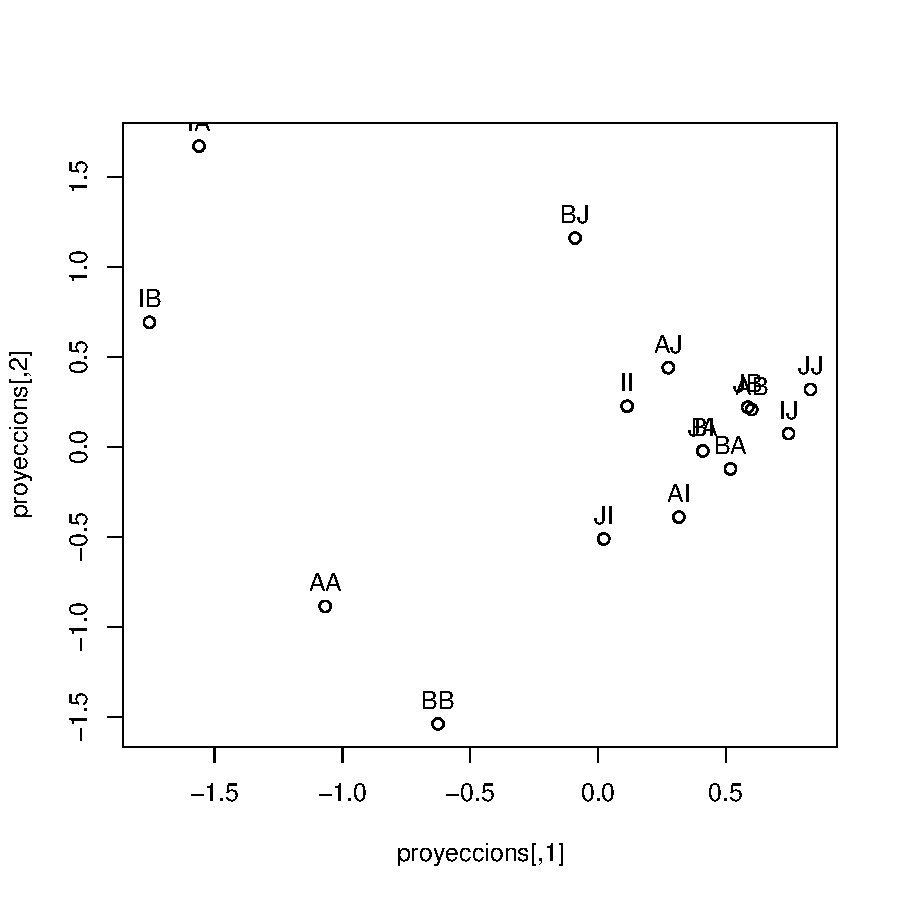
\includegraphics[scale=0.35]{AnCorrFiles.pdf}
\end{center}
}
\end{itemize}
\end{frame}
\subsection{Proyección de las columnas}
\begin{frame}
\frametitle{Proyección de las columnas}
\begin{itemize}
\item<2->{Vamos a realizar el mismo análisis de la matriz de frecuencias relativas $\vect{F}$ que hemos hecho anteriormente pero ahora por columnas.}
\item<3->{Consideramos las $J$ columnas como $J$ puntos en el espacio $\mathbb{R}^I$.}
\item<4->{El objetivo de nuestro análisis es buscar una representación de estos $J$ puntos en un espacio de dimensión menor que nos permita apreciar sus distancias relativas.}
\item<5->{Debemos tener en cuenta las mismas consideraciones que teníamos por filas.}
\end{itemize}
\end{frame}

\begin{frame}
\frametitle{Proyección de las columnas}
\begin{itemize}
\item<2->{Para obtener la mejor representación bidimensional de las filas de la tabla de contingencia, hay que seguir los pasos siguientes:
\begin{itemize}
\item<4->{Calcular la matriz $\vect{Z}\vect{Z}^\top$ y obtener sus vectores y valores propios. Los valores propios de la matriz anterior son los mismos que los valores propios de la matriz $\vect{Z}^\top\vect{Z}$ calculada anteriormente.}
\item<5->{Tomar los dos vectores propios, $\vect{w}_1$ y $\vect{w}_2$ ligados a los dos mayores valores propios menores que la unidad de esta matriz.}
\item<6->{Calcular las proyecciones siguientes $\vect{D}_c^{-1}\vect{F}^\top\vect{D}_f^{-1/2}\vect{w}_i$, $i=1,2$ y representarlas gráficamente en un espacio bidimensional.}
\end{itemize}}
\end{itemize}
\end{frame}

\begin{frame}
\frametitle{Ejemplo anterior}
\begin{itemize}
\item<2->{La matriz $\vect{Z}\vect{Z}^\top$ valdrá:
{\tiny
$$
\left(
\begin{array}{r@{}r@{}r@{}r@{}r@{}r@{}r@{}r@{}r@{}r@{}r@{}r@{}r@{}r@{}r@{}r}
0.25, &   0.02, &   0.07, &   0.02, &   0.02, &   0.24, &   0.04, &   0.00, &   0.06, &   0.15, &   0.06, &   0.00, &   0.04, &   0.02, &   0.10, &   0.00 \\
0.02, &   0.10, &   0.04, &   0.08, &   0.04, &   0.00, &   0.07, &   0.03, &   0.00, &   0.03, &   0.07, &   0.07, &   0.07, &   0.07, &   0.08, &   0.12 \\
0.07, &   0.04, &   0.12, &   0.06, &   0.09, &   0.12, &   0.06, &   0.04, &   0.00, &   0.00, &   0.08, &   0.07, &   0.06, &   0.07, &   0.03, &   0.08 \\
0.02, &   0.08, &   0.06, &   0.12, &   0.09, &   0.03, &   0.08, &   0.08, &   0.10, &   0.02, &   0.09, &   0.09, &   0.08, &   0.06, &   0.06, &   0.09 \\
0.02, &   0.04, &   0.09, &   0.09, &   0.16, &   0.06, &   0.12, &   0.02, &   0.00, &   0.03, &   0.03, &   0.09, &   0.12, &   0.06, &   0.03, &   0.04 \\
0.24, &   0.00, &   0.12, &   0.03, &   0.06, &   0.35, &   0.03, &   0.00, &   0.00, &   0.00, &   0.08, &   0.03, &   0.03, &   0.00, &   0.10, &   0.00 \\
0.04, &   0.07, &   0.06, &   0.08, &   0.12, &   0.03, &   0.14, &   0.02, &   0.00, &   0.05, &   0.03, &   0.05, &   0.14, &   0.09, &   0.05, &   0.04 \\
0.00, &   0.03, &   0.04, &   0.08, &   0.02, &   0.00, &   0.02, &   0.13, &   0.16, &   0.00, &   0.10, &   0.03, &   0.02, &   0.05, &   0.00, &   0.06 \\
0.06, &   0.00, &   0.00, &   0.10, &   0.00, &   0.00, &   0.00, &   0.16, &   0.35, &   0.17, &   0.10, &   0.00, &   0.00, &   0.00, &   0.00, &   0.00 \\
0.15, &   0.03, &   0.00, &   0.02, &   0.03, &   0.00, &   0.05, &   0.00, &   0.17, &   0.36, &   0.00, &   0.00, &   0.05, &   0.03, &   0.03, &   0.00 \\
0.06, &   0.07, &   0.08, &   0.09, &   0.03, &   0.08, &   0.03, &   0.10, &   0.10, &   0.00, &   0.14, &   0.07, &   0.03, &   0.06, &   0.06, &   0.13 \\
0.00, &   0.07, &   0.07, &   0.09, &   0.09, &   0.03, &   0.05, &   0.03, &   0.00, &   0.00, &   0.07, &   0.11, &   0.05, &   0.04, &   0.05, &   0.12 \\
0.04, &   0.07, &   0.06, &   0.08, &   0.12, &   0.03, &   0.14, &   0.02, &   0.00, &   0.05, &   0.03, &   0.05, &   0.14, &   0.09, &   0.05, &   0.04 \\
0.02, &   0.07, &   0.07, &   0.06, &   0.06, &   0.00, &   0.09, &   0.05, &   0.00, &   0.03, &   0.06, &   0.04, &   0.09, &   0.11, &   0.03, &   0.10 \\
0.10, &   0.08, &   0.03, &   0.06, &   0.03, &   0.10, &   0.05, &   0.00, &   0.00, &   0.03, &   0.06, &   0.05, &   0.05, &   0.03, &   0.11, &   0.07 \\
0.00, &   0.12, &   0.08, &   0.09, &   0.04, &   0.00, &   0.04, &   0.06, &   0.00, &   0.00, &   0.13, &   0.12, &   0.04, &   0.10, &   0.07, &   0.23
\end{array}
\right)
$$
}}
\item<3->{Los valores propios de la matriz anterior son:
$$
\begin{array}{r}
1.00,  0.57,  0.52,  0.37,  0.24,  0.12,  0.11,  0.00,\\  0.00,  0.00,  0.00,  0.00,  0.00,  0.00,  0.00,  0.00.
\end{array}
$$ Obsérvese que los valores propios no nulos ya estaban calculados al hacer el análisis por filas.}
\end{itemize}
\end{frame}

\begin{frame}
\frametitle{Ejemplo anterior}
\begin{itemize}
\item<2->{Los vectores propios correspondientes a los valores propios $0.57$ y $0.52$ son:
{\tiny $$
\vect{w}=\begin{pmatrix}
0.41 & 0.35 \\
-0.18 & -0.06 \\
-0.11 & 0.14 \\
-0.10 & -0.17 \\
-0.18 & 0.04 \\
0.24 & 0.61 \\
-0.14 & 0.01 \\
0.02 & -0.29 \\
0.46 & -0.51 \\
0.52 & -0.21 \\
-0.04 & -0.09 \\
-0.22 & -0.02 \\
-0.14 & 0.01 \\
-0.17 & -0.07 \\
-0.01 & 0.16 \\
-0.32 & -0.13 
\end{pmatrix}
$$}}
\end{itemize}
\end{frame}

\begin{frame}
\frametitle{Ejemplo anterior}
\begin{itemize}
\item<2->{La matriz $\vect{D}_c^{-1}\vect{F}^\top\vect{D}_f^{-1/2}$ vale en nuestro caso:
{\tiny
$$
\left(
\begin{array}{r@{}r@{}r@{}r@{}r@{}r@{}r@{}r@{}r@{}r@{}r@{}r@{}r@{}r@{}r@{}r}
0.00, &   0.00, &   0.00, &   0.70, &   0.00, &   0.00, &   0.00, &   1.10, &   1.80, &   0.00, &   0.70, &   0.00, &   0.00, &   0.00, &   0.00, &   0.00 \\
0.00, &   0.64, &   0.00, &   0.50, &   0.00, &   0.00, &   0.00, &   0.00, &   0.00, &   0.00, &   0.50, &   0.64, &   0.00, &   0.00, &   0.64, &   1.00 \\
0.00, &   0.00, &   0.49, &   0.44, &   0.98, &   0.44, &   0.49, &   0.00, &   0.00, &   0.00, &   0.00, &   0.56, &   0.49, &   0.00, &   0.00, &   0.00 \\
0.00, &   0.28, &   0.49, &   0.22, &   0.24, &   0.00, &   0.24, &   0.35, &   0.00, &   0.00, &   0.44, &   0.28, &   0.24, &   0.56, &   0.00, &   0.65 \\
0.32, &   0.41, &   0.00, &   0.32, &   0.36, &   0.00, &   0.71, &   0.00, &   0.00, &   0.41, &   0.00, &   0.00, &   0.71, &   0.41, &   0.41, &   0.00 \\
1.05, &   0.00, &   0.39, &   0.00, &   0.00, &   1.40, &   0.00, &   0.00, &   0.00, &   0.00, &   0.35, &   0.00, &   0.00, &   0.00, &   0.45, &   0.00 \\
0.87, &   0.00, &   0.00, &   0.00, &   0.00, &   0.00, &   0.00, &   0.00, &   1.13, &   2.25, &   0.00, &   0.00, &   0.00, &   0.00, &   0.00, &   0.00
\end{array}
\right)
$$
}
}
\item<3->{Las proyecciones $\vect{D}_c^{-1}\vect{F}^\top\vect{D}_f^{-1/2}\vect{w}$ calculadas por columnas valen:
$$
\begin{pmatrix}
0.75 & -1.43 \\
-0.65 & -0.21 \\
-0.43 & 0.29 \\
-0.61 & -0.24 \\
-0.10 & 0.01 \\
0.70 & 1.31 \\
2.03 & -0.75 
\end{pmatrix}
$$}
\end{itemize}
\end{frame}

\begin{frame}
\frametitle{Ejemplo anterior}
\begin{itemize}
\item<2->{La representación gráfica de las proyecciones anteriores es:
\begin{center}
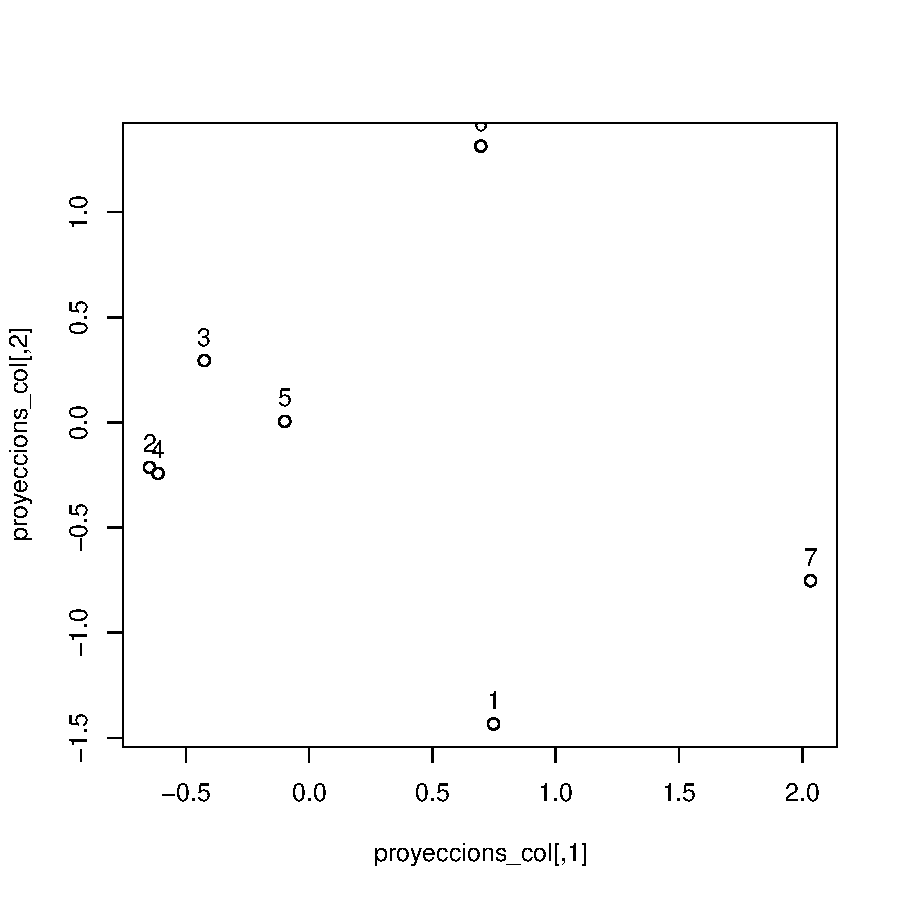
\includegraphics[scale=0.35]{AnCorrColumnes.pdf}
\end{center}}
\end{itemize}
\end{frame}
\begin{frame}
\frametitle{Ejemplo anterior}
\begin{itemize}
\item<2->{En el gráfico anterior se puede observar las similitudes o las diferencias del genotipo entre las crías de rata y las ratas adultas que las crían con diferente porcentaje de aumento de peso al cabo de 28 días. }
\item<3->{Por ejemplo, vemos que las crías de rata y ratas adultas con porcentaje de aumento de peso en segundo y en cuarto lugar tienen un genotipo muy parecido.}
\item<4->{En cambio, la mayor diferencia entre el genotipo de las crías y las ratas adultas se encuentra en las crías de rata con porcentaje de aumento de peso en primer y sexto lugar.}
\end{itemize}
\end{frame}
\subsection{Análisis conjunto}
\begin{frame}
\frametitle{Análisis conjunto}
\begin{itemize}
\item<2->{Debido a la simetría del problema, conviene representar conjuntamente las proyecciones de las filas y las columnas en el mismo gráfico.}
\item<3->{Antes de dar los pasos para hacer tal representación conviene tener en cuenta que
\begin{itemize}
\item<4->{si $\vect{v}$ es vector propio de la matriz $\vect{Z}^\top\vect{Z}$ de valor propio $\lambda$, entonces $\vect{Z}\vect{v}$ es vector propio de la matriz $\vect{Z}\vect{Z}^\top$ del mismo valor propio y} \item<5->{viceversa: si $\vect{w}$ es vector propio de la matriz $\vect{Z}\vect{Z}^\top$ de valor propio $\lambda$, entonces $\vect{Z}^\top\vect{w}$ es vector propio de la matriz $\vect{Z}^\top\vect{Z}$ del mismo valor propio.}
\end{itemize}}
\end{itemize}
\end{frame}

\begin{frame}
\frametitle{Análisis conjunto}
\begin{itemize}
\item<2->{Para hacer la representación conjunta de las proyecciones de las filas y las columnas hay que realizar los pasos siguientes:\begin{itemize}
\item<3->{Se calcula la matriz de frecuencias relativa $\vect{F}$.}
\item<4->{Se calcula la matriz estandarizada $\vect{Z}$.}
\item<5->{Se busca de las dos matrices siguientes, $\vect{Z}^\top\vect{Z}$ o  $\vect{Z}\vect{Z}^\top$ la que tenga menor dimensión. Supongamos para fijar ideas que es la matriz $\vect{Z}^\top\vect{Z}$. Se calculan los dos valores propios menores que~$1$ más grandes de la matriz anterior. Sean $\vect{v}_1$ y $\vect{v}_2$ los dos vectores propios asociados a los dos valores propios anteriores. La proyección de las filas vendrá dada por $\vect{D}_f^{-1/2}\vect{Z}\vect{v}_i$, $i=1,2$.}
\item<6->{Sean $\vect{w}_i = \vect{Z}\vect{v}_i$, $i=1,2$ los vectores propios de la matriz $\vect{Z}\vect{Z}^\top$ asociados a los valores propios anteriores. La proyección de las columnas vendrá dada por: 
$\vect{D}_c^{-1/2}\vect{Z}^\top\vect{w}_i$, $i=1,2$.} 
\end{itemize}}
\end{itemize}
\end{frame}

\begin{frame}
\frametitle{Ejemplo anterior}
\begin{itemize}
\item<2->{En el ejemplo anterior la matriz de menor dimensión era $\vect{Z}^\top\vect{Z}$ ($7\times 7$).}
\item<3->{Los valores propios a considerar eran: $0.57$ y $0.52$.}
\item<4->{Los vectores propios eran:$$
\begin{pmatrix}
-0.28 & 0.57 \\
0.29 & 0.10 \\
0.20 & -0.15 \\
0.42 & 0.17 \\
0.06 & -0.00 \\
-0.37 & -0.74 \\
-0.69 & 0.27 
\end{pmatrix}
$$}
\end{itemize}
\end{frame}

\begin{frame}
\frametitle{Ejemplo anterior}
\begin{itemize}
\item<2->{La proyección de las filas era:{\tiny $$
\vect{v}=\begin{pmatrix}
-1.07 & -0.89 \\
0.60 & 0.21 \\
0.32 & -0.39 \\
0.28 & 0.44 \\
0.52 & -0.12 \\
-0.63 & -1.54 \\
0.41 & -0.02 \\
-0.09 & 1.16 \\
-1.56 & 1.67 \\
-1.75 & 0.69 \\
0.11 & 0.23 \\
0.75 & 0.07 \\
0.41 & -0.02 \\
0.59 & 0.22 \\
0.02 & -0.51 \\
0.83 & 0.32 
\end{pmatrix}
$$}
}
\end{itemize}
\end{frame}
\begin{frame}
\frametitle{Ejemplo anterior}
\begin{itemize}
\item<2->{Busquemos ahora los vectores propios de la matriz $\vect{Z}\vect{Z}^\top$: $\vect{w}_i = \vect{Z}\vect{v}_i$, donde $\vect{v}_i$ son los vectores propios hallados anteriormente por columnas:
{\tiny $$
\vect{w}=\begin{pmatrix}
-0.31 & -0.25 \\
0.13 & 0.05 \\
0.08 & -0.10 \\
0.08 & 0.13 \\
0.13 & -0.03 \\
-0.18 & -0.44 \\
0.10 & -0.01 \\
-0.02 & 0.21 \\
-0.35 & 0.37 \\
-0.39 & 0.15 \\
0.03 & 0.06 \\
0.17 & 0.02 \\
0.10 & -0.01 \\
0.13 & 0.05 \\
0.00 & -0.11 \\
0.24 & 0.09 \\
\end{pmatrix}
$$}}
\end{itemize}
\end{frame}

\begin{frame}
\frametitle{Ejemplo anterior}
\begin{itemize}
\item<2->{Las proyecciones de las columnas será la matriz $\vect{D}_c^{-1/2}\vect{Z}^\top\vect{w}$:
$$\begin{pmatrix}
-0.56 & 1.03 \\
0.49 & 0.15 \\
0.32 & -0.21 \\
0.46 & 0.17 \\
0.07 & -0.00 \\
-0.52 & -0.95 \\
-1.53 & 0.54 \\
\end{pmatrix}$$
}
\end{itemize}
\end{frame}
\begin{frame}
\frametitle{Ejemplo anterior}
\begin{itemize}
\item<2->{En el gráfico siguiente se puede ver la proyección conjunta donde en rojo están las proyecciones por filas y en negro, las proyecciones por columnas:
\begin{center}
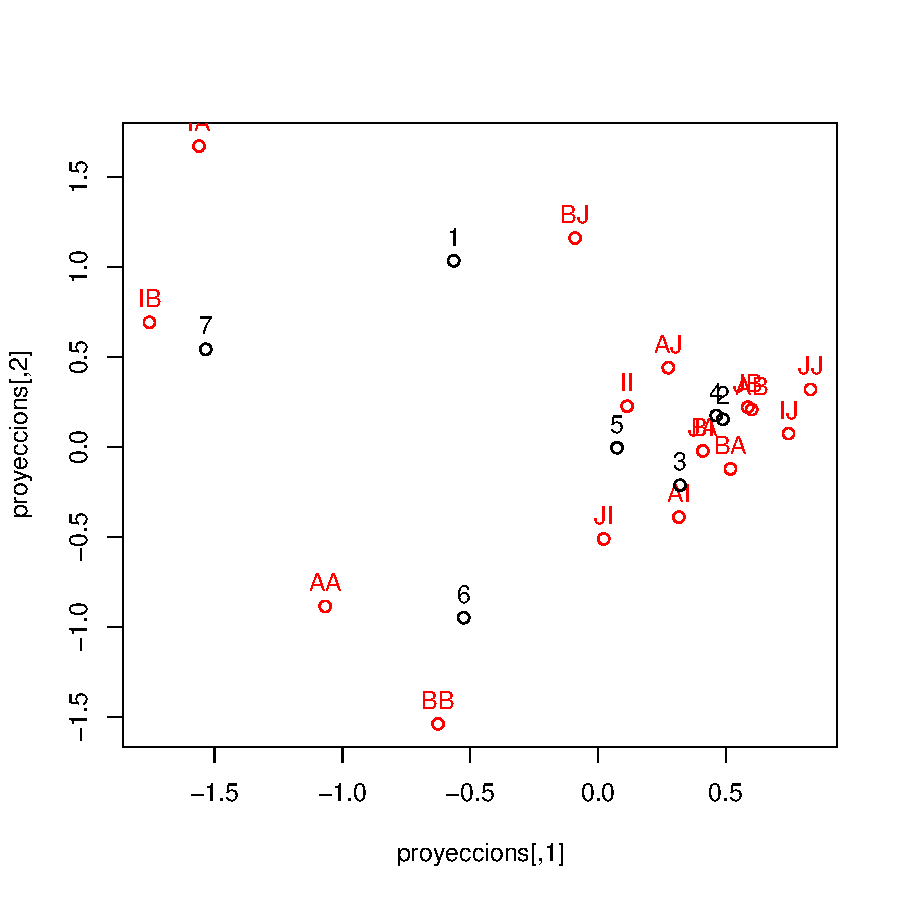
\includegraphics[scale=0.5]{AnCorrConjunta.pdf}
\end{center}}
\end{itemize}
\end{frame}
